\documentclass[11pt,a4paper]{scrartcl}
\usepackage[utf8]{inputenc}
\usepackage[english]{babel}
\usepackage{graphicx}
\usepackage{geometry}
\usepackage{fancyhdr}
\usepackage[table]{xcolor}
\usepackage{mathtools}
\usepackage{logicpuzzle}
\usepackage{listings}
\usepackage{hyperref}
\usepackage[toc,page]{appendix}
\hypersetup{
    colorlinks,
    citecolor=black,
    filecolor=black,
    linkcolor=black,
    urlcolor=black
}

 
\usepackage{fancyhdr} % Custom headers and footers
\pagestyle{fancyplain} % Makes all pages in the document conform to the custom headers and footers
\fancyhead{} % No page header - if you want one, create it in the same way as the footers below
\fancyfoot[L]{} % Empty left footer
\fancyfoot[C]{} % Empty center footer
\fancyfoot[R]{\thepage} % Page numbering for right footer
\renewcommand{\headrulewidth}{0pt} % Remove header underlines
\renewcommand{\footrulewidth}{0pt} % Remove footer underlines
\setlength{\headheight}{13.6pt} % Customize the height of the header
%
\lstset{ %
  basicstyle=\footnotesize,        % the size of the fonts that are used for the code
  breakatwhitespace=false,         % sets if automatic breaks should only happen at whitespace
  breaklines=true,                 % sets automatic line breaking
  captionpos=b,                    % sets the caption-position to bottom
  deletekeywords={...},            % if you want to delete keywords from the given language
  extendedchars=true,              % lets you use non-ASCII characters; for 8-bits encodings only, does not work with UTF-8
  frame=single,                    % adds a frame around the code
  keepspaces=true,                 % keeps spaces in text, useful for keeping indentation of code (possibly needs columns=flexible)
                keywordstyle=\color{blue},
                stringstyle=\color{red},
                commentstyle=\color{green},
                morecomment=[l][\color{magenta}]{\#},
  language=C,                 % the language of the code
  showspaces=false,                % show spaces everywhere adding particular underscores; it overrides 'showstringspaces'
  showstringspaces=false,          % underline spaces within strings only
  showtabs=false,                  % show tabs within strings adding particular underscores
  tabsize=4,                       % sets default tabsize to 2 spaces
}

\begin{document}
\lstset{language=Prolog,basicstyle=\footnotesize}
\renewcommand\lstlistingname{Code}
\DeclarePairedDelimiter{\ceil}{\lceil}{\rceil}
\definecolor{lgray}{gray}{0.65}
\definecolor{llgray}{gray}{0.90}

\newcommand{\horrule}[1]{\rule{\linewidth}{#1}} % Create horizontal rule command with 1 argument of height

\title{
\normalfont \normalsize
\textsc{KU Leuven} \\ [25pt] % Your university, school and/or department name(s)
\horrule{0.5pt} \\[0.4cm] % Thin top horizontal rule
\huge SORTES: DHCP Relay Agent \\ % The assignment title
\horrule{2pt} \\[0.5cm] % Thick bottom horizontal rule
}
 
\author{Bart Verhoeven \& Arne Van der Stappen} % Your name
 
\date{\normalsize December 31, 2014} % Today's date or a custom date
 
\maketitle % Print the title

\tableofcontents

\newpage

\section{User guide \label{sec:userguide}}
When the board is started up, it will act as a DHCP relay agent. More information about DHCP, and DHCP relay agents can be found on \href{http://en.wikipedia.org/wiki/Dynamic_Host_Configuration_Protocol} {\textbf{Wikipedia}}.

\subsection{Relay Agent configuration}
This relay agent has a static IP address (\textit{192.168.97.60/24}), and is configured to be able to work in the \textit{192.168.97.0/24} subnet. The relay agent itself is preconfigured and should work out of the box once the router and DHCP server are configured as below.

\subsection{DHCP Server configuration}
In order for this relay agent to work, the user needs to set up his own DHCP server. This server should be located in the \textit{192.168.96.0/24} subnet, with \textit{192.168.96.2/24} as ip address. These settings are hardcoded, and can be changed in Main.h if necessary. The server needs to be configured to be able to give out ip addresses in the subnet of the relay agent (\textit{192.168.97.60/24}). The relay agent will now relay DHCP messages from his subnet to the DHCP server.

\subsection{Router configuration}
The router between the two networks should have the NAT feature disabled.

\section{System Engineer guide}
\subsection{Compile}
To compile the program, simply type \textbf{\textit{make DHCPRelay}} while in the source root.

\subsection{Upload to Pic}
To upload the program to the pic, upload \textbf{\textit{main.hex}} using tftp as described in \href{http://www.foditic.org/SORTES\_14/missions/picUnixE.php}{\textbf{PIC development in C on UNIX howto}}.

\subsection{Tests}
To test the board, you can enable a DHCP client in the subnet of the DHCP relay agent. This client should now be assigned an IP address by the DHCP server.\\

The following tests have been run to confirm the correct working of the agent:
\begin{itemize}
\item A single PC connecting to the network and requesting a new IP
\item Multiple PC's connecting to the network at the same time and requesting a new IP
\item A PC with a static IP connecting to the network
\item A PC reconnecting to the network and requesting their old IP
\item A PC connected to the network for a longer period of time and renewing its lease
\end{itemize}

\section{Design Decisions}

The code of this relay agent was produced by translating ASG diagrams \ref{fig:asg} and \ref{fig:asgRelaying} to C.
As described in the ASG diagram, the relay agent has two components. One component receives ip packages, the other component sends ip packages. TODO VERDERE UITLEG

\begin{figure}
	\centering
	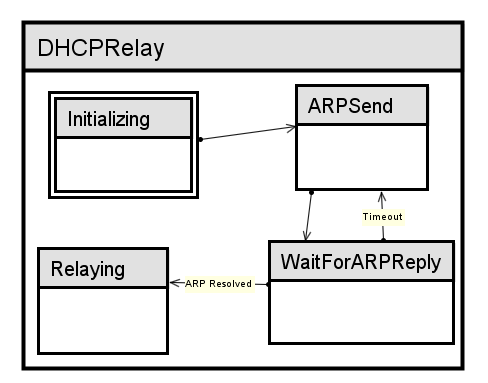
\includegraphics[width=1.0\textwidth]{../img/dhcprelay-asg.png}
	\caption{ASG diagram of the DHCP Relay Agent.\label{fig:asg}}
\end{figure}

\begin{figure}
	\centering
	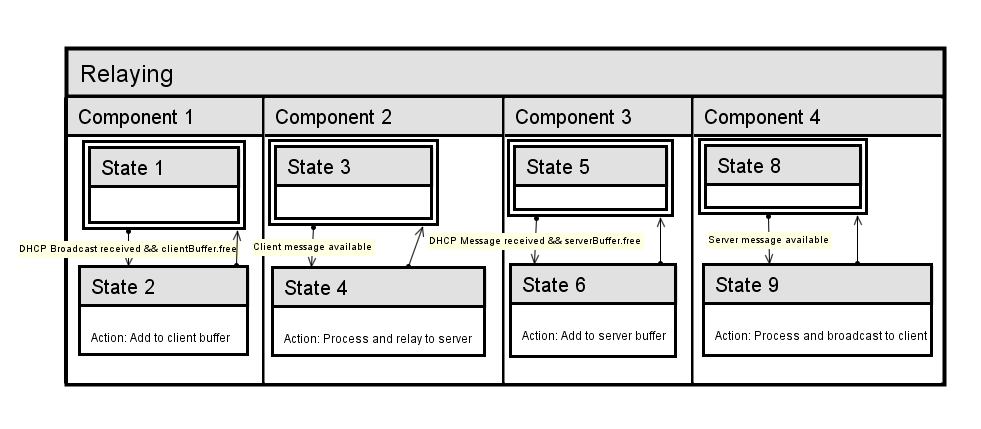
\includegraphics[width=1.0\textwidth]{../img/relaying-asg.png}
	\caption{ASG diagram of the Relaying state.\label{fig:asgRelaying}}
\end{figure}

\subsection{Seperate Client/Server components}

\subsection{Seperate Receive/Process components}

\subsection{Buffer size}
The internal buffers from which the processing-components of the application consume and for which the receiving-components of the application produce dhcp packages, have a size of one. This means that each pair of components (receiver-processor) of the application are tightly coupled. The consumer component has to consume the last packet before the producer can produce a new one. This limitation makes sure there is enough memory on the processor to hold the buffer. While this may seem like a heavy limitation, it is really not. The TCP/IP stack implementation provided does also work with only one packet.\\
Given enough memory, this buffer could easily be extended to contain more than one message. This would not affect the workings of the components 

\subsection{Immeadiate state changes}

\newpage

\appendix
\section{Code}

\subsection{main.h}
\lstinputlisting[language=C]{../src/Main.h}

\subsection{main.c}
\lstinputlisting[language=C]{../src/Main.c}

\subsection{messageProcessor.h}
\lstinputlisting[language=C]{../src/messageProcessor.h}

\subsection{messageProcessor.c}
\lstinputlisting[language=C]{../src/messageProcessor.c}

\subsection{DHCPBuffer.h}
\lstinputlisting[language=C]{../src/DHCPBuffer.h}

\subsection{DHCPBuffer.c}
\lstinputlisting[language=C]{../src/DHCPBuffer.c}

\subsection{receiver.h}
\lstinputlisting[language=C]{../src/receiver.h}

\subsection{receiver.c}
\lstinputlisting[language=C]{../src/receiver.c}

\subsection{Debug.h}
\lstinputlisting[language=C]{../src/Debug.h}

\end{document}